\section{Memory Model}
\subsection{Java}
In Java sind \textbf{atomare} Schreibe- und Leseinstruktionen nur für Primitive Datentypen bis 32-bit und Objekt-Referenzen garantiert. Long und Double Typen sind nur mit \underline{volatile} atomar.

Nur atomar bedeutet nicht, dass Thread B die Änderung auch mit bekommt. \textbf{Visibility} synchronisiert lese/schreibe Zugriff von volatile Variablen.

\begin{center}
	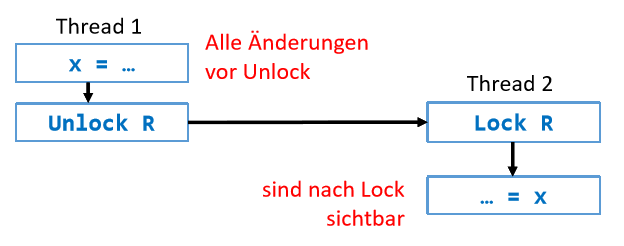
\includegraphics[width=0.6\columnwidth]{Images/visibility}
\end{center}

In Java sind zudem alle Synchronisations-Instruktionen total \textbf{ordered}, in c\# nicht! d.H in Java funktioniert folgendes Beispiel, in c\# nicht.
\begin{lstlisting}
volatile boolean a = false, b = false;

// Thread 1					// Thread 2
a = true;						b = true;
while(!b) {}				while(!a) {}
\end{lstlisting}

In c\# kann dies verhindert werden mit Thread.MemoryBarrier(), dies verhindert die Umordnung.
\begin{lstlisting}
volatile boolean a = false, b = false;

// Thread 1								// Thread 2
a = true;									b = true;
Thread.MemoryBarrier();		Thread.MemoryBarrier();
while(!b) {}							while(!a) {}
\end{lstlisting}


\subsection{Atomare Operationen}
In Java sind \textit{Atomic*} für *Integer, *Long, *Referenzen diversen Funktionen getAndSet(), addAndGet(), getAndAdd() oder compareAndSet(expect, update) etc atomar.

